\chapter{Resultados y discusión}
\label{chap:resultados}
Se presentan los resultados obtenidos con las representaciones y los modelos descritos en el Capítulo~\ref{chap:metodologia}. Se separan la validación geométrica, la evaluación de clasificación y las mediciones de costo, porque corresponden a conjuntos de observaciones y alcances diferentes. Las tablas se elaboraron a partir de los archivos de resultados versionados; las figuras de este capítulo se generaron a partir de esos mismos registros. Los ejemplos ilustrativos de la metodología no se utilizaron como sustitutos de las mediciones del conjunto de prueba.

\section{Validación de las representaciones tridimensionales}
\label{sec:resultados-representaciones}
La muestra controlada incluyó diez modelos: un objeto de entrenamiento y uno de prueba de cada categoría \texttt{airplane}, \texttt{car}, \texttt{chair}, \texttt{sofa} y \texttt{table}. Se obtuvieron veinte registros al considerar las dos resoluciones. El resumen de ejecución informó diez modelos exitosos y ninguno fallido; las comprobaciones registraron equivalencia correcta y ausencia de errores de integridad. Esta evidencia corresponde a la muestra controlada, no a una auditoría individual de los $12\,311$ modelos.

La Tabla~\ref{tab:geometria-resultados} resume los conteos y tamaños de esta muestra. La ocupación es la proporción de hojas ocupadas respecto a las celdas de la resolución equivalente; los promedios se calcularon sobre diez objetos por resolución.
\begin{table}[htbp]\centering\small
\caption{Promedios de la muestra controlada (diez objetos por resolución). Los tamaños NPZ se expresan en KiB y la ocupación en porcentaje. Elaboración propia.}\label{tab:geometria-resultados}
\setlength{\tabcolsep}{4pt}
\begin{tabular}{@{}lrrrrr@{}}\toprule
$R$ & Nodos & Hojas & Ocupación (\%) & NPZ octree & NPZ denso \\\midrule
32 & 2\,015,1 & 1\,523,1 & 4,65 & 17,02 & 12,90 \\
64 & 7\,605,1 & 5\,590,0 & 2,13 & 40,16 & 44,34 \\
\bottomrule\end{tabular}\end{table}


El crecimiento del número de hojas no implicó reservar todos los elementos de la rejilla densa. Sin embargo, una estructura de objetos Python introduce referencias y sobrecarga que no están presentes en una estimación binaria de sus arreglos. Por ello, la compacidad del archivo NPZ no demuestra por sí sola un menor pico de memoria durante la construcción. Asimismo, la compresión del tensor denso puede aprovechar regiones repetidas; la comparación pertinente depende de si se estudia memoria de trabajo, carga binaria o almacenamiento comprimido.

La Tabla~\ref{tab:construccion-costos} presenta los indicadores de construcción registrados para esta muestra. La memoria transitoria se interpreta según la instrumentación del primer objetivo y no como el conjunto de trabajo de Windows utilizado después en inferencia.
\begin{table}[htbp]\centering\small
\caption{Promedios de construcción del octree en la muestra controlada, con diez objetos por resolución. El pico transitorio registrado, la estimación de estructura Python y la carga binaria se mantienen separados. Elaboración propia.}\label{tab:construccion-costos}
\begin{tabular}{@{}rrrrr@{}}\toprule
$R$ & Tiempo (ms) & Pico (MiB) & Python (MiB) & Binaria (KiB) \\\midrule
32 & 139,70 & 1,29 & 0,94 & 35,90 \\
64 & 515,11 & 3,80 & 3,49 & 134,16 \\\bottomrule\end{tabular}\end{table}

Las diferencias entre columnas muestran por qué la carga binaria no sustituye una medición de memoria de construcción. Los tiempos son promedios por objeto de esta muestra y no una extrapolación medida del procesamiento completo de ModelNet40. La carga binaria registrada incluye el alcance definido por el generador de métricas y debe distinguirse de los 18 bytes por nodo de los cuatro arreglos estructurales aislados.

La comprobación específica de \texttt{chair\_0001} verificó las representaciones antes y después de guardar y cargar. En $32^3$ se registraron 762 hojas ocupadas y $1\,121$ nodos; en $64^3$ se registraron $2\,573$ hojas ocupadas y $3\,694$ nodos totales. La diferencia máxima registrada en las normales fue del orden de $1{,}19\times10^{-7}$, compatible con la tolerancia de la comprobación numérica. Este objeto se mantuvo como caso ilustrativo de verificación geométrica.

En el inventario completo se registraron $12\,311$ archivos por resolución. Los octrees ocuparon $203{,}33$ MB en $32^3$ y $436{,}62$ MB en $64^3$, equivalentes a promedios de $16{,}13$ y $34{,}63$ KiB por objeto. El almacenamiento creció aproximadamente $2{,}15$ veces; este cociente describe archivos comprimidos de este conjunto y no una ley general de complejidad del octree.

\section{Resultados del enfoque clásico}
\label{sec:resultados-hce}
La auditoría registrada no encontró columnas constantes ni valores no finitos en el entrenamiento oficial. El descriptor $o_1$ presentó variabilidad y se conservó. Los contratos persistidos no excluyeron ninguna de las 17 o 18 columnas del esquema base; la exclusión de $o_0$ ya formaba parte de la definición analítica. La comprobación documental posterior sobre los $8\,858$ índices de ajuste reconstruidos tampoco encontró columnas constantes ni valores no finitos. En ambas resoluciones, $o_1$ varió entre $25\,\%$ y $100\,\%$. Por tanto, restringir este diagnóstico a ajuste conservó los mismos índices y dimensiones, sin detectar un cambio de características que exigiera repetir los entrenamientos.

Los registros complementarios de correspondencia fila--objeto incluyeron $9\,843$ identificadores únicos en cada resolución: $8\,858$ de ajuste y 985 de validación. La comparación con el manifiesto de Net5 produjo cero diferencias tanto en los identificadores como en sus posiciones dentro de cada subconjunto. También coincidieron las categorías y el orden de objetos entre las resoluciones $32^3$ y $64^3$. Las huellas consignadas en los registros correspondieron a los archivos HCE examinados, mientras que las dos ejecuciones de Net5 registraron la misma huella del manifiesto. Por tanto, las relaciones aportadas son consistentes con una partición común entre HCE y Net5.

Los CSV declararon una coincidencia única de descriptores para cada una de las $9\,843$ filas de ambas resoluciones. Este resultado se reporta conforme a los registros suministrados; durante la revisión documental no se volvió a ejecutar la comparación de descriptores contra los octrees originales. La verificación realizada cubrió la integridad interna de las relaciones y su concordancia con el manifiesto, y quedó registrada en \protect\path{verificacion_relaciones_hce.json}. Los registros complementan los NPZ de características, que no almacenan identificadores de objeto por fila.

Los clasificadores clásicos utilizaron 17 características en $32^3$ y 18 en $64^3$, conforme al contrato de características. El SVM seleccionado empleó núcleo de base radial, parámetro de penalización 10 y la regla \texttt{scale} para la anchura del núcleo en ambas resoluciones. El Bosque Aleatorio conservó cien árboles. El escalador del SVM formó parte del modelo persistido, de modo que la predicción reutilizó la transformación ajustada durante el entrenamiento.

El SVM pasó de $75{,}93\,\%$ a $77{,}19\,\%$ de exactitud; el bosque pasó de $76{,}38\,\%$ a $77{,}19\,\%$. En $64^3$ ambos acertaron $1\,905$ objetos, pero sus F1 macro fueron distintos y sus predicciones no fueron idénticas. La igualdad de la exactitud agregada no implica que los métodos cometan los mismos errores. Las exactitudes balanceadas, inferiores a las globales, muestran que el comportamiento promedio por categoría fue menos favorable que el sugerido por el conteo total de aciertos.

\section{Resultados de Net5}
\label{sec:resultados-net5}
Net5 alcanzó $82{,}21\,\%$ en $32^3$ y $83{,}23\,\%$ en $64^3$, con $2\,029$ y $2\,054$ aciertos, respectivamente. Las épocas seleccionadas fueron la 25 y la 19; las ejecuciones finalizaron en las épocas 45 y 39 por el criterio de parada anticipada. Las mejores exactitudes de validación fueron $84{,}77\,\%$ y $85{,}48\,\%$. La Figura~\ref{fig:curvas-finales} muestra la evolución de ajuste y validación, para distinguir la selección del modelo de su evaluación posterior en prueba.
\begin{figure}[htbp]\centering
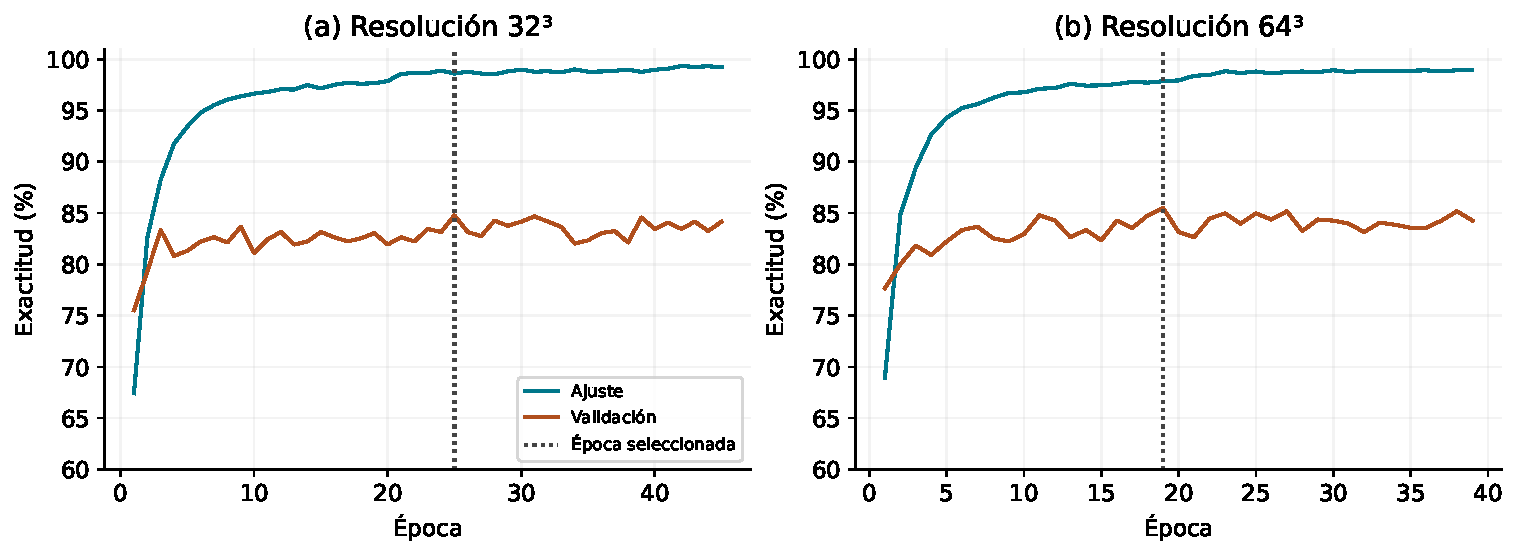
\includegraphics[width=\textwidth]{Figuras/cierre_curvas.pdf}
\caption{Evolución de la exactitud de Net5 en ajuste y validación: (a) resolución $32^3$ y (b) resolución $64^3$. Las líneas verticales señalan las épocas seleccionadas. Elaboración propia a partir de los historiales completos; la prueba no intervino en esta selección.}\label{fig:curvas-finales}
\end{figure}
La separación entre las curvas evidencia una capacidad elevada para ajustar los objetos de entrenamiento sin alcanzar el mismo desempeño en validación. La parada anticipada limitó la prolongación del ajuste, pero no eliminó esa diferencia. No se evaluó una familia de capacidades de red ni distintas semillas de entrenamiento; por tanto, estos resultados corresponden a la configuración descrita y no al máximo desempeño posible de las redes basadas en octrees.

\section{Comparación del desempeño de clasificación}
\label{sec:comparacion-clasificacion}
La Tabla~\ref{tab:clasificacion-final} presenta los resultados de prueba de los tres métodos para facilitar su comparación bajo el mismo conjunto de objetos. Se incluyen los aciertos y errores junto con métricas que distinguen el desempeño global del promedio entre categorías.
\begin{table}[H]\centering\small
\caption{Evaluación sobre 2\,468 objetos por configuración. Exactitud (A), exactitud balanceada (AB) y promedios F1 expresados en porcentaje. Elaboración propia.}\label{tab:clasificacion-final}
\setlength{\tabcolsep}{4pt}
\begin{tabular}{@{}lrrrrrrr@{}}\toprule
Método & $R$ & Aciertos & Errores & A & AB & F1 macro & F1 pond. \\\midrule
SVM & 32 & 1\,874 & 594 & 75,93 & 66,24 & 65,82 & 75,47 \\
Bosque & 32 & 1\,885 & 583 & 76,38 & 67,64 & 67,72 & 75,43 \\
Net5 & 32 & 2\,029 & 439 & 82,21 & 75,81 & 74,93 & 81,99 \\
SVM & 64 & 1\,905 & 563 & 77,19 & 68,86 & 68,47 & 76,91 \\
Bosque & 64 & 1\,905 & 563 & 77,19 & 67,80 & 68,53 & 76,35 \\
Net5 & 64 & 2\,054 & 414 & 83,23 & 77,29 & 77,23 & 83,38 \\
\bottomrule\end{tabular}\end{table}


Net5 superó al SVM en $6{,}28$ puntos porcentuales en $32^3$ y en $6{,}04$ en $64^3$. Frente al bosque, la diferencia fue de $5{,}83$ y $6{,}04$ puntos. El F1 macro también fue mayor para Net5: $74{,}93\,\%$ y $77{,}23\,\%$, frente a valores entre $65{,}82\,\%$ y $68{,}53\,\%$ en los métodos clásicos. La ventaja no se restringió, por tanto, a la exactitud global.

La Tabla~\ref{tab:intervalos-finales} presenta los intervalos de exactitud para los modelos fijos. Su amplitud describe la incertidumbre del remuestreo de prueba y no la estabilidad entre entrenamientos.
\begin{table}[htbp]\centering\small
\caption{Intervalos percentiles del 95\,\% para la exactitud, mediante 2\,000 remuestreos del conjunto de prueba. Límites en porcentaje; no incluyen variabilidad del entrenamiento. Elaboración propia.}\label{tab:intervalos-finales}
\begin{tabular}{@{}lrrr@{}}\toprule
Método & $R$ & Límite inferior (\%) & Límite superior (\%) \\\midrule
SVM & 32 & 74,19 & 77,63 \\
Bosque & 32 & 74,76 & 78,04 \\
Net5 & 32 & 80,71 & 83,71 \\
SVM & 64 & 75,41 & 78,81 \\
Bosque & 64 & 75,53 & 78,81 \\
Net5 & 64 & 81,77 & 84,72 \\\bottomrule\end{tabular}\end{table}

Los límites de Net5 quedaron por encima de los de los clásicos en estas observaciones. La comparación emparejada se examinó mediante los contrastes siguientes, en lugar de utilizar el solapamiento de intervalos como prueba de igualdad.

La Tabla~\ref{tab:contrastes-finales} presenta las discordancias emparejadas y los valores de probabilidad de los nueve contrastes. Se informan sin corrección por multiplicidad, como se estableció en la metodología.
\begin{table}[htbp]\centering\small
\caption{Comparaciones emparejadas. Las dos columnas centrales cuentan aciertos exclusivos del primer y segundo método; los valores de probabilidad son individuales, sin ajuste por multiplicidad. Elaboración propia.}\label{tab:contrastes-finales}
\setlength{\tabcolsep}{4pt}
\begin{tabular}{@{}lrrr@{}}\toprule
Comparación & Solo primero & Solo segundo & $p$ \\\midrule
Net5 vs SVM (32) & 297 & 142 & $1,1\times10^{-13}$ \\
Net5 vs Bosque (32) & 282 & 138 & $1,8\times10^{-12}$ \\
Bosque vs SVM (32) & 178 & 167 & 0,590 \\
Net5 vs SVM (64) & 289 & 140 & $5,3\times10^{-13}$ \\
Net5 vs Bosque (64) & 293 & 144 & $8,7\times10^{-13}$ \\
Bosque vs SVM (64) & 158 & 158 & 1,000 \\
SVM: $64^3$ frente a $32^3$ & 110 & 79 & 0,029 \\
Bosque: $64^3$ frente a $32^3$ & 102 & 82 & 0,161 \\
Net5: $64^3$ frente a $32^3$ & 125 & 100 & 0,109 \\
\bottomrule\end{tabular}\end{table}


Los contrastes de Net5 frente a los métodos clásicos registraron valores inferiores a $10^{-11}$. No se detectó una diferencia entre bosque y SVM al nivel nominal utilizado. La diferencia entre resoluciones del SVM registró un valor de $0{,}029$, que debe interpretarse con cautela por la multiplicidad de contrastes. Las diferencias entre resoluciones del bosque y de Net5 no alcanzaron el umbral nominal; este resultado no prueba igualdad entre resoluciones.

La Figura~\ref{fig:recall-final} presenta la sensibilidad por categoría y configuración. Las seis matrices de confusión completas se incluyen en el Anexo~\ref{anexo:confusiones}; allí se mantiene la normalización por fila para comparar categorías con soportes distintos.
\begin{figure}[p]\centering
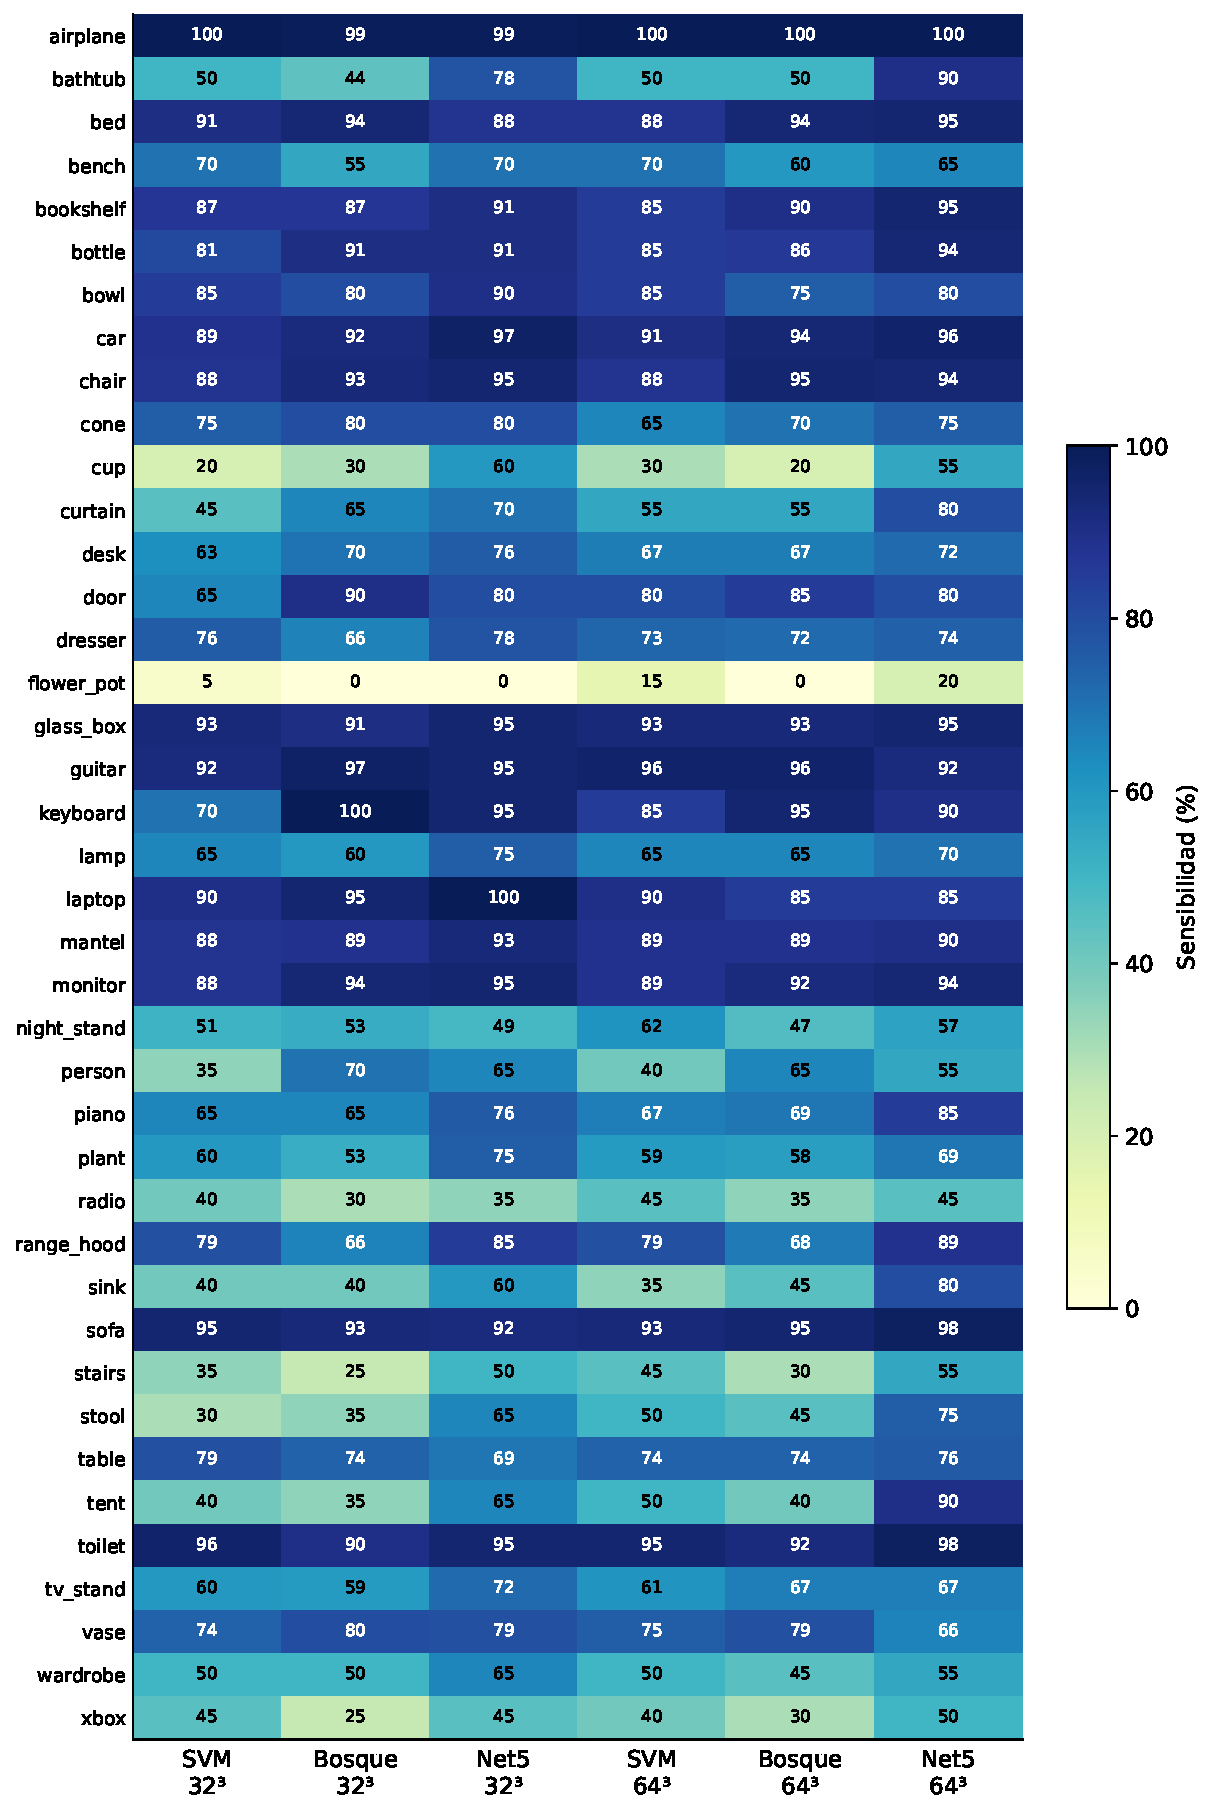
\includegraphics[width=0.94\textwidth,height=0.79\textheight,keepaspectratio]{Figuras/cierre_sensibilidad.pdf}
\caption{Sensibilidad por categoría de los tres métodos en $32^3$ y $64^3$, expresada en porcentaje. Cada columna representa una configuración y cada fila una categoría oficial. Elaboración propia a partir de las predicciones de los $2\,468$ objetos de prueba.}\label{fig:recall-final}
\end{figure}
Entre las confusiones recurrentes se encontraron \texttt{night\_stand} con \texttt{dresser}, \texttt{table} con \texttt{desk} y \texttt{bottle} con \texttt{vase}. Para Net5, los errores de \texttt{table} hacia \texttt{desk} disminuyeron de 28 a 17 al aumentar la resolución, mientras que los de \texttt{dresser} hacia \texttt{night\_stand} aumentaron de 13 a 18. La mejora global no fue uniforme entre categorías ni entre pares de clases. La similitud geométrica de estos objetos constituye una explicación plausible, pero no se realizó una intervención experimental que aislara su causa.

Los tres métodos acertaron simultáneamente $1\,616$ objetos en $32^3$ y $1\,651$ en $64^3$; todos fallaron en 250 y 226 objetos, respectivamente. Net5 acertó de forma exclusiva 166 y 179 objetos. A su vez, en 189 y 188 casos Net5 falló y al menos un clasificador clásico acertó. Estos conteos muestran complementariedad de errores, aunque no constituyen el resultado de un ensamblaje entrenado ni justifican atribuirle la exactitud de un selector ideal.

\section{Comparación del costo computacional}
\label{sec:comparacion-costo}
La Tabla~\ref{tab:latencia-final} presenta las medianas de carga, extracción o preparación geométrica y predicción o propagación, junto con la mediana y el percentil 95 del agregado por objeto. Se conservaron los límites de instrumentación desde el NPZ, incluida la exclusión del armado de lote en el caso GPU de Net5 indicada en la metodología.
\begin{table}[htbp]\centering\small
\caption{Latencia por objeto en la muestra de 400 objetos. Los componentes y el agregado se expresan en milisegundos. El agregado GPU de Net5 excluye el armado del lote; el de CPU lo incluye. Elaboración propia a partir de la medición principal.}\label{tab:latencia-final}
\setlength{\tabcolsep}{3pt}
\begin{tabular}{@{}lr rrr rr@{}}\toprule
& & \multicolumn{3}{c}{Medianas por componente (ms)} & \multicolumn{2}{c}{Agregado (ms)} \\
\cmidrule(lr){3-5}\cmidrule(l){6-7}
Método & $R$ & Carga & \shortstack{Extracción/\\preparación} & \shortstack{Predicción/\\propagación} & Mediana & P95 \\\midrule
SVM & 32 & 8,32 & 5,02 & 0,82 & 14,32 & 34,60 \\
Bosque & 32 & 8,32 & 5,02 & 5,88 & 19,66 & 40,76 \\
Net5 GPU & 32 & 7,30 & 37,55 & 5,91 & 52,09 & 105,39 \\
Net5 CPU & 32 & 7,30 & 37,55 & 102,65 & 148,54 & 312,37 \\
SVM & 64 & 27,56 & 23,04 & 0,82 & 52,74 & 118,77 \\
Bosque & 64 & 27,56 & 23,04 & 5,77 & 57,68 & 123,82 \\
Net5 GPU & 64 & 24,91 & 187,90 & 11,81 & 230,10 & 462,94 \\
Net5 CPU & 64 & 24,91 & 187,90 & 334,87 & 549,10 & 1\,090,24 \\
\bottomrule\end{tabular}
\par\smallskip\begin{minipage}{\textwidth}\footnotesize
Para SVM y Bosque, la segunda etapa corresponde a extracción HCE y la tercera a predicción con el clasificador. Para Net5, corresponden a preparación geométrica y propagación en el dispositivo indicado. P95: percentil 95. Las medianas de componentes no se suman para obtener la mediana del agregado; este se calcula por objeto antes de resumirlo.\end{minipage}
\end{table}


Los intervalos instrumentados de HCE y Net5 no abarcaron exactamente las mismas operaciones; por ello, no se utilizaron sus cocientes para establecer una ventaja directa de velocidad entre ambos enfoques. La preparación geométrica de Net5 tuvo medianas de $37{,}55$ y $187{,}90$ ms, superiores a las de su propagación GPU, de $5{,}91$ y $11{,}81$ ms. En los métodos clásicos, la predicción aislada del SVM permaneció alrededor de $0{,}82$ ms, mientras que la carga y extracción aumentaron con la resolución. Estos resultados identifican etapas costosas; no atribuyen toda la latencia al clasificador.

La Tabla~\ref{tab:memoria-final} distingue la memoria adicional, la memoria total del proceso y la memoria GPU asignada y reservada. Los picos corresponden a la muestra efectiva de cien objetos de tres categorías.
\begin{table}[htbp]\centering\small
\caption{Memoria observada sobre cien objetos de tres categorías, en MiB. RAM adicional respecto a la base; VRAM asignada y reservada por PyTorch. Elaboración propia.}\label{tab:memoria-final}
\setlength{\tabcolsep}{4pt}
\begin{tabular}{@{}lrrrr@{}}\toprule
Método & $R$ & RAM adicional & RAM total & VRAM asig. / res. \\\midrule
SVM & 32 & 40,4 & 161,4 & -- \\
Bosque & 32 & 267,6 & 388,2 & -- \\
Net5 GPU & 32 & 728,9 & 1\,308,9 & 137,7 / 300,0 \\
Net5 CPU & 32 & 272,2 & 852,4 & -- \\
SVM & 64 & 42,2 & 163,0 & -- \\
Bosque & 64 & 266,0 & 386,9 & -- \\
Net5 GPU & 64 & 821,5 & 1\,401,9 & 420,6 / 1\,972,0 \\
Net5 CPU & 64 & 734,2 & 1\,314,4 & -- \\
\bottomrule\end{tabular}\end{table}


El SVM presentó el menor incremento de RAM observado. El bosque requirió aproximadamente 266--268 MiB adicionales y Net5 en GPU, 729--821 MiB en la medición principal. Parte de la diferencia entre memoria total y adicional procede del entorno de bibliotecas y del contexto de ejecución. Estas magnitudes no equivalen al tamaño de los pesos ni a la memoria de un octree individual.

La Tabla~\ref{tab:modelos-finales} presenta el almacenamiento y la complejidad de los modelos conservados. Se separa esta comparación de la memoria de inferencia porque la representación serializada y la residente tienen costos distintos.
\begin{table}[htbp]\centering\small
\caption{Tamaño de los modelos en MB decimales y complejidad estructural. Los conteos de complejidad son adimensionales. Elaboración propia.}\label{tab:modelos-finales}
\setlength{\tabcolsep}{4pt}
\begin{tabular}{@{}lrrr@{}}\toprule
Método & $R$ & Archivo (MB) & Complejidad \\\midrule
SVM & 32 & 4,43 & 5\,765 vectores \\
Bosque & 32 & 137,73 & 358\,494 nodos / 100 árboles \\
Net5 & 32 & 34,20 & 8\,547\,456 parámetros \\
SVM & 64 & 4,39 & 5\,662 vectores \\
Bosque & 64 & 137,15 & 356\,984 nodos / 100 árboles \\
Net5 & 64 & 34,20 & 8\,547\,456 parámetros \\
\bottomrule\end{tabular}\end{table}


El bosque produjo archivos aproximadamente 31 veces mayores que los del SVM, sin registrar una ventaja de exactitud en $64^3$. Net5 mantuvo prácticamente constante el tamaño del archivo entre resoluciones porque el número de parámetros fue el mismo. El aumento del costo de ejecución de Net5 se relacionó con las representaciones y operaciones intermedias, no con un incremento del número de pesos aprendidos.

La Tabla~\ref{tab:entrenamiento-final} presenta el tiempo de entrenamiento requerido por el quinto objetivo y separa la preparación HCE de los ajustes de los clasificadores. Cada fila identifica la unidad, la naturaleza medida o estimada y las operaciones incluidas.
\begin{table}[htbp]\centering\small
\caption{Tiempos de preparación HCE y entrenamiento por resolución. Se distingue cada etapa, su unidad y la naturaleza del valor. Elaboración propia a partir de los resúmenes de entrenamiento y la estimación documentada.}\label{tab:entrenamiento-final}
\setlength{\tabcolsep}{4pt}
\begin{tabularx}{\textwidth}{@{}>{\raggedright\arraybackslash}p{3.2cm}rrl>{\raggedright\arraybackslash}X@{}}\toprule
Etapa & $32^3$ & $64^3$ & Unidad & Naturaleza y alcance \\\midrule
Carga y extracción HCE & 2,53 & 9,23 & min & Estimada: extrapolación de carga del NPZ y extracción a los $9\,843$ objetos del entrenamiento oficial. \\ \addlinespace
Búsqueda y ajuste del SVM & 15,70 & 17,30 & s & Medida: búsqueda con validación cruzada y ajuste final; características ya disponibles. \\ \addlinespace
Ajuste del Bosque Aleatorio & 0,49 & 0,49 & s & Medida: ajuste con las características disponibles; no incluye su extracción. \\ \addlinespace
Entrenamiento de Net5 & 173,31 & 476,86 & min & Medida: duración acumulada de las épocas, incluida validación; 45 épocas en $32^3$ y 39 en $64^3$. \\ \addlinespace
\bottomrule\end{tabularx}
\end{table}


La estimación HCE extrapoló a los $9\,843$ objetos oficiales de entrenamiento la suma de las medias de carga y extracción obtenidas en la muestra de latencia; no constituye el cronometraje de una extracción completa. La búsqueda y el ajuste de los clasificadores clásicos comenzaron con las características disponibles. En Net5 se acumuló la duración de las épocas, incluida la validación, hasta la parada anticipada. Por tanto, estas duraciones permiten identificar el costo de cada etapa documentada, pero no se compararon como intervalos equivalentes ni se sumaron para atribuirles un tiempo experimental completo desde la malla.

La Tabla~\ref{tab:reevaluacion-final} contrasta las latencias y los picos de RAM de la medición principal con la reevaluación del 27 de septiembre. Las predicciones de los seis modelos coincidieron objeto a objeto en los $2\,468$ casos, mientras que las mediciones temporales variaron. El informe de esa ejecución registró 103 pruebas automatizadas aprobadas en el entorno de su autor. Este conteo corresponde al registro conservado y no a una nueva ejecución durante la revisión documental.
\begin{table}[htbp]\centering\small
\caption{Latencia y memoria RAM de la medición principal y la reevaluación del 27 de septiembre de 2026. La latencia corresponde a 400 objetos y la memoria a 100. La variación temporal se calcula respecto a la principal. Elaboración propia a partir de ambos registros.}\label{tab:reevaluacion-final}
\setlength{\tabcolsep}{4pt}
\textbf{(a) Mediana de latencia por objeto}\par\smallskip
\begin{tabular}{@{}lrrrr@{}}\toprule
Método & $R$ & Principal (ms) & Reevaluación (ms) & Variación (\%) \\\midrule
SVM & 32 & 14,32 & 13,61 & -4,94 \\
Bosque & 32 & 19,66 & 18,69 & -4,94 \\
Net5 GPU & 32 & 52,09 & 48,30 & -7,28 \\
Net5 CPU & 32 & 148,54 & 153,20 & 3,14 \\
SVM & 64 & 52,74 & 51,53 & -2,29 \\
Bosque & 64 & 57,68 & 56,78 & -1,57 \\
Net5 GPU & 64 & 230,10 & 217,52 & -5,47 \\
Net5 CPU & 64 & 549,10 & 587,05 & 6,91 \\
\bottomrule\end{tabular}
\par\medskip\textbf{(b) Pico de RAM adicional y total del proceso}\par\smallskip
\begin{tabular}{@{}lr rrrr@{}}\toprule
& & \multicolumn{2}{c}{RAM adicional (MiB)} & \multicolumn{2}{c}{RAM total (MiB)} \\
\cmidrule(lr){3-4}\cmidrule(l){5-6}
Método & $R$ & Principal & Reevaluación & Principal & Reevaluación \\\midrule
SVM & 32 & 40,42 & 40,34 & 161,39 & 161,23 \\
Bosque & 32 & 267,59 & 267,80 & 388,19 & 389,01 \\
Net5 GPU & 32 & 728,94 & 747,82 & 1\,308,91 & 1\,328,07 \\
Net5 CPU & 32 & 272,17 & 273,94 & 852,39 & 853,62 \\
SVM & 64 & 42,15 & 45,80 & 162,96 & 166,53 \\
Bosque & 64 & 266,01 & 266,13 & 386,88 & 386,96 \\
Net5 GPU & 64 & 821,49 & 764,57 & 1\,401,90 & 1\,344,72 \\
Net5 CPU & 64 & 734,21 & 729,83 & 1\,314,35 & 1\,309,95 \\
\bottomrule\end{tabular}
\par\smallskip\begin{minipage}{\textwidth}\footnotesize
RAM adicional: incremento del pico observado sobre la base de cada proceso. RAM total: pico del conjunto de trabajo del proceso. En las filas Net5 GPU se informa RAM del equipo, no VRAM; ambas magnitudes son distintas. Los alcances temporales conservan las salvedades de la Tabla~\ref{tab:latencia-final}.\end{minipage}
\end{table}


La preservación de las predicciones respalda la repetición de la evaluación de los modelos conservados. Las variaciones temporales muestran que una ejecución no fija una constante de rendimiento del equipo. En particular, el aumento de RAM adicional GPU de Net5 entre resoluciones fue de $12{,}7\,\%$ en la corrida principal (de $728{,}94$ a $821{,}49$ MiB) y de $2{,}2\,\%$ en la reevaluación (de $747{,}82$ a $764{,}57$ MiB), como respalda el panel (b) de la Tabla~\ref{tab:reevaluacion-final}; no se estableció un porcentaje estable atribuible únicamente a la resolución.

\section{Análisis de escalabilidad por resolución}
\label{sec:escalabilidad}
Las ganancias de exactitud al pasar de $32^3$ a $64^3$ fueron $1{,}26$ puntos para SVM, $0{,}81$ para bosque y $1{,}01$ para Net5. Representaron 31, 20 y 25 aciertos adicionales, respectivamente. Las medianas temporales se multiplicaron aproximadamente por $3{,}68$, $2{,}93$ y $4{,}42$ para SVM, bosque y Net5 en GPU. Net5 acumuló alrededor de $2{,}75$ veces el tiempo de entrenamiento. Estos cocientes corresponden a las dos resoluciones ensayadas y no constituyen una extrapolación a resoluciones superiores.

Aunque duplicar la resolución de cada eje multiplica por ocho las celdas de una rejilla densa, el archivo comprimido de los octrees completos aumentó aproximadamente $2{,}15$ veces. La reducción de almacenamiento frente al crecimiento cúbico no implica que las operaciones posteriores escalen con el mismo factor: intervienen la cantidad de hojas, la geometría, la preparación de planes y el movimiento de datos.

\section{Compromiso entre desempeño y costo}
\label{sec:compromiso}
La Figura~\ref{fig:compromiso-final} relaciona la exactitud y la latencia mediana para visualizar la decisión entre configuraciones. Esta figura reúne magnitudes presentadas por separado en las tablas. Las líneas permiten examinar el cambio de resolución dentro de cada método; la separación horizontal entre métodos con alcances temporales distintos no se interpreta como una razón comparable de velocidad.
\begin{figure}[htbp]\centering
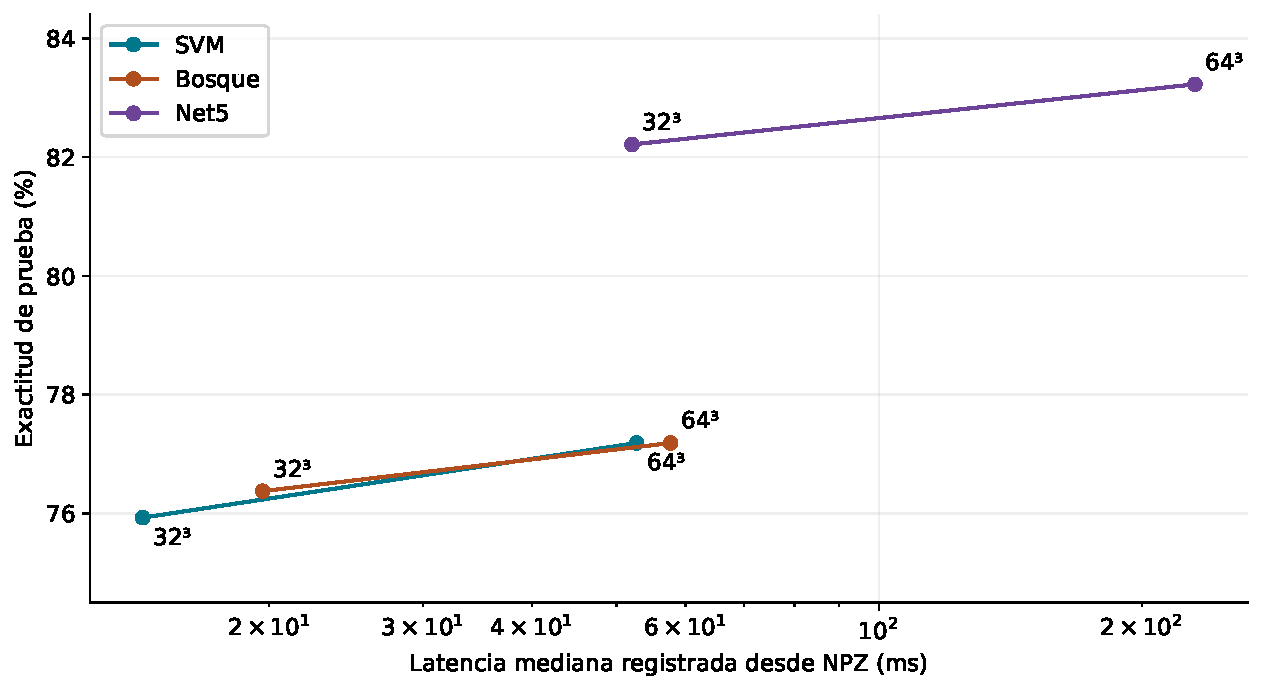
\includegraphics[width=\textwidth]{Figuras/cierre_compromiso.pdf}
\caption{Exactitud de prueba frente a mediana de latencia registrada desde NPZ. Las líneas unen resoluciones de un mismo método; Net5 corresponde a GPU. La abscisa usa escala logarítmica. Su tiempo omite el armado previo del lote, por lo que no representa un tiempo completo desde la malla ni un alcance idéntico al de CPU. Elaboración propia.}\label{fig:compromiso-final}
\end{figure}
Dentro del protocolo común de los dos clasificadores clásicos, SVM en $32^3$ presentó menor latencia y menor incremento de RAM. Su archivo de modelo fue también el menor entre las configuraciones evaluadas. Los tiempos agregados de Net5 y HCE no permiten extender esa conclusión a una clasificación global de velocidad, porque sus alcances no son idénticos. Cuando se priorizó exactitud, Net5 en $64^3$ obtuvo el mayor valor. Net5 en $32^3$ superó la exactitud de ambos clásicos en $64^3$ y evitó gran parte del costo de Net5 en alta resolución. La elección depende del costo admisible y de las categorías relevantes; no se identificó una configuración universalmente superior en todas las dimensiones.

\FloatBarrier
\section{Síntesis del cumplimiento y alcance de los objetivos}
\label{sec:sintesis-objetivos}
Antes de la discusión, la Tabla~\ref{tab:sintesis-objetivos} relaciona los objetivos con las evidencias presentadas, su ubicación y los límites de interpretación. Esta síntesis permite comprobar la trazabilidad de los resultados sin sustituir las conclusiones del Capítulo~\ref{chap:conclusiones}.
\begingroup\small\singlespacing
\setlength{\tabcolsep}{3pt}
\renewcommand{\arraystretch}{1.03}
\begin{longtable}{@{}>{\raggedright\arraybackslash}p{1.9cm}>{\raggedright\arraybackslash}p{3.05cm}>{\raggedright\arraybackslash}p{2.15cm}>{\raggedright\arraybackslash}p{2.9cm}>{\raggedright\arraybackslash}p{3.0cm}@{}}
\caption{Síntesis del cumplimiento y alcance de los objetivos. Los títulos abreviados remiten a los objetivos aprobados en la Sección~\ref{sec:objetivos}. Elaboración propia.}\label{tab:sintesis-objetivos}\\
\toprule Objetivo & Evidencia obtenida & Ubicación & Alcance efectivo & Limitaciones de la evidencia \\\midrule\endfirsthead
\multicolumn{5}{l}{\tablename~\thetable\ (continuación)}\\\toprule
Objetivo & Evidencia obtenida & Ubicación & Alcance efectivo & Limitaciones de la evidencia \\\midrule\endhead
\midrule\multicolumn{5}{r}{Continúa en la página siguiente}\\\endfoot
\bottomrule\endlastfoot
General: comparación reproducible & Predicciones, métricas y costos de seis configuraciones; modelos y registros conservados. & Secciones\newline\ref{sec:comparacion-clasificacion}--\ref{sec:compromiso}. & Clasificación de ModelNet40 en dos resoluciones, sobre $2\,468$ objetos de prueba. & Un equipo y una semilla; los alcances de algunos tiempos difieren. \\ \addlinespace
1. Enfoque clásico basado en octree & Representaciones construidas; equivalencia y persistencia verificadas en la muestra; clasificación clásica evaluada. & Secciones~\ref{sec:resultados-representaciones} y~\ref{sec:resultados-hce}; Tablas~\ref{tab:geometria-resultados} y~\ref{tab:construccion-costos}. & Inventario de $12\,311$ octrees por resolución; diez objetos y veinte registros en la validación controlada. & La verificación geométrica de la muestra no equivale a una auditoría exhaustiva del inventario. \\ \addlinespace
2. HCE, SVM y Bosque Aleatorio & Vectores de 17 y 18 componentes; contratos auditados; modelos seleccionados y persistidos. & Sección~\ref{sec:resultados-hce}; Tabla~\ref{tab:clasificacion-final}. & Partición de $8\,858$ objetos de ajuste y 985 de validación; prueba oficial separada. & Asociación fila--objeto respaldada por registros y revisión del programa, sin repetir localmente su ejecución. \\ \addlinespace
3. Net5 basado en octrees & Dos modelos entrenados; historiales y mejores estados conservados; evaluación final. & Sección~\ref{sec:resultados-net5}; Figura~\ref{fig:curvas-finales}; Tabla~\ref{tab:clasificacion-final}. & Mismas particiones documentadas; resoluciones $32^3$ y $64^3$. & Un entrenamiento por configuración; sin estudio de ablación ni variabilidad entre semillas. \\ \addlinespace
4. Protocolo reproducible y trazabilidad & Manifiestos, relaciones HCE, huellas y versiones; seis secuencias de predicción preservadas en la reevaluación. & Secciones~\ref{sec:resultados-hce} y~\ref{sec:comparacion-costo}; Tabla~\ref{tab:reevaluacion-final}. & Repetición de la evaluación de los modelos guardados; 103 pruebas aprobadas según el registro de ejecución. & No constituye reentrenamiento independiente; varían tiempos y memoria entre ejecuciones. \\ \addlinespace
5. Desempeño, costo y escalabilidad & Exactitud, confusiones, intervalos, contrastes, entrenamiento, latencia, memoria y tamaño. & Secciones\newline\ref{sec:comparacion-clasificacion}--\ref{sec:compromiso}; Tablas~\ref{tab:latencia-final}--\ref{tab:reevaluacion-final}; Anexo~\ref{anexo:confusiones}. & Prueba: $2\,468$ objetos; latencia: 400; memoria: 100; comparación entre dos resoluciones. & Extracción HCE estimada; memoria de tres categorías; tiempos con alcances distintos y sin medición de energía. \\
\end{longtable}\endgroup


La evidencia de cumplimiento se circunscribe al componente experimental y a las condiciones especificadas. La disponibilidad de modelos y registros respalda la comparación realizada; no extiende sus conclusiones a otros equipos, conjuntos de datos o modalidades de adquisición.

\section{Discusión general}
\label{sec:discusion-general}
La ventaja de Net5 frente a las características manuales se manifestó tanto en exactitud global como en F1 macro y en los contrastes emparejados de la Tabla~\ref{tab:contrastes-finales}. Los vectores HCE resumieron la ocupación, la distribución espacial y las normales mediante 17 o 18 componentes; Net5 aprendió transformaciones de los atributos conservando relaciones espaciales durante sus bloques convolucionales. Una explicación plausible de la diferencia es que esos resúmenes globales no retienen toda la información discriminante accesible al modelo aprendido. Esta interpretación es coherente con el interés de la literatura por aprender representaciones directamente de datos tridimensionales, mediante octrees o conjuntos de puntos~\parencite{riegler2017,qi2017}. Sin embargo, no se realizó una ablación que aislara el efecto de las características, la arquitectura o la capacidad del clasificador. La evidencia respalda la ventaja de esta configuración de Net5 sobre los dos modelos HCE evaluados, no una superioridad universal del aprendizaje profundo.

El aumento de resolución produjo ganancias pequeñas frente a su costo: Net5 obtuvo 25 aciertos adicionales, equivalentes a $1{,}01$ puntos porcentuales, mientras su latencia GPU registrada aumentó $4{,}42$ veces y el entrenamiento $2{,}75$ veces. El contraste exacto de McNemar entre resoluciones registró $p=0{,}109$ y no alcanzó el umbral nominal de $0{,}05$. Este resultado no demuestra equivalencia ni ausencia de una mejora; indica que, para estos modelos fijos y los pares observados, no se obtuvo evidencia suficiente para declarar una diferencia bajo ese criterio. Tampoco permite establecer una resolución óptima general, dado que solo se estudiaron dos resoluciones y una semilla de entrenamiento.

Existe un antecedente pertinente en OctNet: en el experimento de clasificación de ModelNet40 de su material suplementario, el desempeño mejoró hasta aproximadamente $32^3$ y no continuó aumentando al elevar la resolución, manteniendo fijo el número de parámetros~\parencite{riegler2017}. La mejora limitada observada aquí es conceptualmente consistente con ese comportamiento: un mayor detalle espacial no garantiza una ganancia proporcional en clasificación. La comparación es conceptual, porque las implementaciones, los atributos, las configuraciones y las condiciones experimentales no son idénticos. No se presenta este trabajo como una reproducción cuantitativa de las exactitudes o los tiempos de OctNet, ni el contraste no significativo como una demostración independiente de saturación.

La relación entre dispersión y costo exige separar almacenamiento y ejecución. OctNet explota la dispersión mediante octrees poco profundos para concentrar representación y cómputo en regiones relevantes~\parencite{riegler2017}. En este trabajo, el almacenamiento comprimido del inventario aumentó $2{,}15$ veces al duplicar la resolución por eje, frente al factor ocho del número de celdas de una rejilla densa. Ese cociente no mide por sí mismo un ahorro respecto a un tensor denso comprimido: intervienen el formato y la compresión. Tampoco determina el tiempo de cálculo. Las medianas de preparación geométrica de Net5 superaron las de propagación GPU en ambas resoluciones (Tabla~\ref{tab:latencia-final}), lo que muestra que conservar una estructura dispersa no elimina el costo de organizarla para las operaciones de la red.

Los modelos clásicos ofrecen un compromiso distinto: reducen la representación a vectores pequeños y realizan la clasificación una vez disponibles esas características. El SVM presentó menor latencia y menor incremento de RAM que el bosque bajo el protocolo común de HCE, mientras que el bosque ocupó más espacio sin mejorar la exactitud en $64^3$. Estas observaciones favorecen al SVM dentro de esa comparación concreta. Entre HCE y Net5, en cambio, las diferencias de alcance temporal impiden construir una clasificación directa de velocidad a partir de los agregados. La reevaluación preservó las predicciones, pero modificó las mediciones de recursos; por ello, un resultado estable de clasificación no implica que la latencia o el pico de memoria sean constantes del modelo.

La motivación del Grupo de Óptica y Tratamiento de Señales de la Escuela de Física de la Universidad Industrial de Santander se relaciona con el volumen de información de la reconstrucción tridimensional en metrología óptica. Los resultados proporcionan evidencia computacional sobre representación y clasificación en ese contexto de interés. No demuestran mejoras en incertidumbre metrológica, precisión de reconstrucción ni clasificación de mediciones ópticas reales, porque la evaluación se restringió a objetos de ModelNet40.

\section{Amenazas a la validez y limitaciones experimentales}
\label{sec:limitaciones-experimentales}
La validez interna se apoyó en el manifiesto conservado de Net5, los registros complementarios de correspondencia fila--objeto de HCE, la selección mediante validación y la evaluación emparejada. La coincidencia de identificadores y posiciones fue comprobada documentalmente. La asociación por descriptores se sustentó en los CSV suministrados
y en la revisión del programa
\protect\path{trazabilidad_filas_hce.py}, que implementa la
comparación binaria de los vectores recalculados con los almacenados.
Esta comprobación posterior no se repitió de forma independiente
durante la revisión documental. Sin embargo, se realizó un solo entrenamiento por configuración y semilla. Los intervalos por remuestreo del conjunto de prueba no capturan esa fuente de variabilidad. Los nueve contrastes no incluyeron corrección por comparaciones múltiples y sus resultados se interpretaron con ese alcance.

La medición de recursos tuvo limitaciones concretas. La muestra de memoria cubrió solo tres categorías; el muestreo cada 2 ms pudo omitir picos más cortos y el conjunto de trabajo incluye componentes del entorno. El tiempo GPU omitió el armado del lote, mientras que el de CPU lo incluyó. Los tiempos no incluyeron construir el octree desde la malla. La extracción HCE de entrenamiento se estimó. El experimento de CPU utilizó un hilo, por lo que no representa una implementación optimizada para todos los núcleos. Tampoco se midió energía consumida.

La validez externa quedó limitada a un equipo, un sistema operativo, ModelNet40 y dos resoluciones. No se evaluaron escaneos ruidosos, oclusiones, variaciones de pose fuera del protocolo ni otros conjuntos de datos. La muestra geométrica de diez modelos no se convirtió en una afirmación de auditoría exhaustiva de los $12\,311$ objetos. Finalmente, las diferencias entre clases sugieren hipótesis geométricas que requerirían estudios controlados adicionales; no se presentaron como causas demostradas.
